% Chapter VI core fragment; requires amsmath, amssymb, hyperref.
% Designed for a two-column parent document; no floats or wide equations.
\section{Quantum routes and physical records}
\label{sec:quantum-records}
\noindent\textbf{Evidence status.} The calculations below are consequences of standard finite-dimensional quantum mechanics. Born probabilities, Hilbert-space composition, and quantum instruments are premises. The SAM contribution at this stage is a proposed interpretation and a specification of what a substrate write must implement, not a new probability law or an experimentally distinct prediction.

The route language of Unified Volume I, \S5, separates an unresolved alternative from a physical record. Its useful content becomes testable only after the record carrier, decoder, accessible domain, and retention interval are declared. A route can carry phase without leaving a readable mark. Conversely, correlations can suppress local interference even when no observer can read their remote carrier. Accessibility therefore qualifies the \emph{record available to a domain}; it does not switch ordinary quantum entanglement or decoherence on and off.

\subsection{A controlled marker and its observable fringe}
Let $S$ be a two-route system with orthogonal states $|0\rangle,|1\rangle$, and let $M$ be a marker initially in $|m\rangle$. Write $q=1-p$, $0\leq p\leq1$, and prepare
\begin{equation}
 |\psi\rangle_S=\sqrt p\,|0\rangle
       +e^{i\phi}\sqrt q\,|1\rangle .
\end{equation}
A path-preserving marker coupling has the form
\begin{equation}
\begin{gathered}
U=|0\rangle\langle0|\otimes U_0
       +|1\rangle\langle1|\otimes U_1,
 \\
 |m_j\rangle=U_j|m\rangle .
\end{gathered}
\end{equation}
The joint state and overlap convention are
\begin{align}
 |\Psi\rangle&=\sqrt p\,|0\rangle|m_0\rangle
       +e^{i\phi}\sqrt q\,|1\rangle|m_1\rangle,\\
 \gamma&=\langle m_1|m_0\rangle .
\end{align}
Tracing out $M$, rather than assuming a collapse, gives
\begin{equation}
 \rho_S=\begin{pmatrix}
 p&\sqrt{pq}\,e^{-i\phi}\gamma\\
 \sqrt{pq}\,e^{i\phi}\gamma^*&q
 \end{pmatrix}.
 \label{eq:record-reduced}
\end{equation}
For a balanced output analyser with projectors onto
$|\!\pm_\theta\rangle=(|0\rangle\pm e^{i\theta}|1\rangle)/\sqrt2$,
the Born rule yields
\begin{equation}
 P_\pm(\theta)=\tfrac12\pm\sqrt{pq}\,
   \operatorname{Re}[e^{i(\theta-\phi)}\gamma].
 \label{eq:record-fringe}
\end{equation}
Thus the scanned single-port visibility is
\begin{equation}
 V=\frac{P_{\max}-P_{\min}}{P_{\max}+P_{\min}}
   =2\sqrt{pq}\,|\gamma|.
 \label{eq:record-visibility}
\end{equation}
These expressions assume a lossless two-route preparation, a balanced analyser, a phase scan, and no outcome-dependent filtering. Unequal route populations already limit $V$ without a marker. A global phase in the overlap shifts the fringe; its magnitude controls the contrast. A change in contrast is consequently not, by itself, proof of a durable record.

The action-phase interface remains the ordinary one: for two coherent routes, $\Delta\phi=(S_1-S_0)/\hbar$. An $A$-dependent action must specify its Lagrangian, integration parameter, and units before it predicts a fringe shift. The schematic symbol $L_A$ in the source text supplies no independent microscopic Hamiltonian and does not derive the Born rule. In particular, probabilities continue to govern subsequent measurements after a record has formed; ``before the write'' describes the proposed accounting language, not a restriction on the applicability of quantum probability.


\begin{figure*}[t]
\centering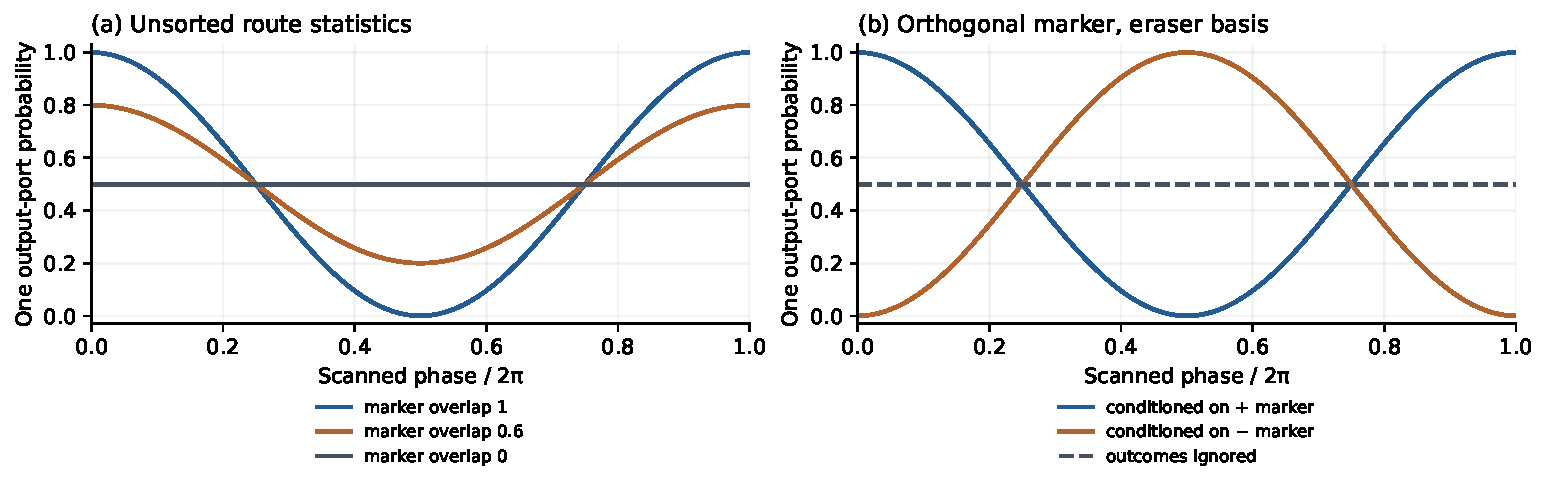
\includegraphics[width=.9\textwidth]{vi_source/record_fringes.pdf}
\caption{Exact balanced two-route comparator. (a) Real marker overlap changes unsorted interference through $P_+=(1+\gamma\cos\varphi)/2$. (b) For orthogonal markers, measuring the complementary marker basis gives two conditional fringes, each with probability one half. Ignoring that outcome yields the unchanged flat marginal. These analytic finite-system curves illustrate the stated protocol; they are not measured SAM data or an original-field simulation.}
\label{fig:record-fringes}
\end{figure*}
\subsection{Distinguishability, with the priors retained}
Consider the operational task of guessing a route from its marker, given priors $p,q$. For any binary POVM $E_0,E_1$ on $M$,
\begin{equation}
\begin{gathered}
P_{\rm guess}=p\,\operatorname{Tr}(E_0\rho_0)
          +q\,\operatorname{Tr}(E_1\rho_1),
 \\
 \rho_j=|m_j\rangle\langle m_j|.
\end{gathered}
\end{equation}
Set $H=p\rho_0-q\rho_1$. Since $E_1=I-E_0$,
maximizing $q+\operatorname{Tr}(E_0H)$ selects the positive spectral subspace of $H$. Hence
\begin{equation}
\begin{gathered}
P_{\rm guess}^{\rm opt}=\tfrac12(1+D),
 \\
 D=\|p\rho_0-q\rho_1\|_1 .
\end{gathered}
\label{eq:weighted-helstrom}
\end{equation}
This is weighted Helstrom distinguishability,\cite{BarnettCroke2009} not the unweighted trace distance unless $p=q=1/2$. On the span of the two pure markers, $\operatorname{Tr}H=p-q$ and
$\det H=-pq(1-|\gamma|^2)$. The two eigenvalues have opposite signs or one is zero, so
\begin{equation}
\begin{gathered}
D=\sqrt{1-4pq|\gamma|^2},\\
 D^2+V^2=1.
\end{gathered}
\label{eq:record-duality}
\end{equation}
Identical marker states give $D=|p-q|$: success then comes only from the prior imbalance. Orthogonal markers give $D=1$, $V=0$. Equation~\eqref{eq:record-duality} is an equality for this pure joint state with full marker access and the specified analyser. It is not an unrestricted equality for every apparatus. It belongs to the established two-way duality framework; see Englert.\cite{Englert1996}

There is a short general proof of the relevant inequality. Let $\rho_{SM}$ be any joint state and purify it with $E$. For $0<p<1$ the purification can be written
\begin{equation}
 |\Omega\rangle=\sqrt p\,|0\rangle|u\rangle_{ME}
                 +\sqrt q\,|1\rangle|v\rangle_{ME},
\end{equation}
with normalized conditional vectors. If $c=\langle0|\rho_S|1\rangle$, then $c=\sqrt{pq}\langle v|u\rangle$ and the same analyser gives $V=2|c|$. Weighted pure-state discrimination on $ME$ gives
$D_{ME}=\sqrt{1-4|c|^2}$. Partial trace is a trace-norm contraction on Hermitian operators, yielding
\begin{equation}
\begin{gathered}
D_M\leq D_{ME},\\
 D_M^2+V^2\leq1.
\end{gathered}
\label{eq:mixed-duality}
\end{equation}
The endpoints $p=0,1$ follow directly. This proof also covers a restricted accessible subsystem of the marker. It does not license comparing visibility in one postselected ensemble with distinguishability in another. These are the standard channel and discrimination conventions.\cite{Watrous2018}

\subsection{Reversal, erasure, and inaccessible markers}
An exact reversible two-qubit fixture uses $|m\rangle=|0\rangle$,
$U_0=I$, and
\begin{equation}
 U_1=R(\alpha)=\begin{pmatrix}
 \cos\alpha&-\sin\alpha\\ \sin\alpha&\cos\alpha
 \end{pmatrix}.
\end{equation}
Then $\gamma=\cos\alpha$. At $p=1/2$, $V=|\cos\alpha|$ and $D=|\sin\alpha|$. At $\alpha=\pi/2$ the marker is orthogonal and the reduced route state has no coherence. Applying the \emph{joint controlled inverse} $U^\dagger$ before analysis restores $|\psi\rangle|0\rangle$ and the original visibility. This is a reversal of the correlation-generating interaction. A marker-only unitary cannot accomplish it, since it preserves $\langle m_1|m_0\rangle$.

A quantum eraser is a different operation. For the orthogonal marker, measure $M$ in $|\!\pm\rangle_M=(|0\rangle\pm|1\rangle)/\sqrt2$. Each outcome has probability $1/2$ and prepares the conditional route state
\begin{equation}
 |\psi_\pm\rangle=\sqrt p\,|0\rangle
                   \pm e^{i\phi}\sqrt q\,|1\rangle .
\end{equation}
Its fringe visibility is $2\sqrt{pq}$, but the two fringes are shifted by $\pi$. Averaging their distributions cancels the interference. Conditional coincidence sorting requires the marker outcome; it does not restore an unconditional remote fringe. Outcome-dependent feed-forward can align the phases, but uses a communicated outcome and an operation on $S$. This distinction is central to the original quantum-eraser proposal of Scully and Dr\"uhl and to conditional coincidence experiments.\cite{ScullyDruhl1982,Kim2000}

Environmental copies constrain reversal. For branch states of the factorized form $|m_j\rangle|e_j\rangle$, the coherence multiplier is
\begin{equation}
 \gamma_{ME}=\langle m_1|m_0\rangle
                  \langle e_1|e_0\rangle .
\end{equation}
Reversing the controlled $S$--$M$ coupling while leaving $E$ intact does not remove the environmental factor. Orthogonal $|e_j\rangle$ maintain zero local coherence even when $E$ is inaccessible. Generic environmental states need not factorize; the purification argument above replaces this product formula in that case. No assertion about a gravitational horizon follows merely from tracing out $E$.

More generally, let $\Lambda_M$ be any trace-preserving local channel, including an unread measurement or reset. For every bipartite state,
\begin{align}
 \rho'_S&=\operatorname{Tr}_M[(I\otimes\Lambda_M)(\rho_{SM})]
            =\rho_S,\\
 T(\rho'_S,\rho_S)&=\tfrac12\|\rho'_S-\rho_S\|_1=0.
\end{align}
The equality follows from $\Lambda_M^*(I)=I$: every local expectation on $S$ is unchanged. Thus no route-only POVM can reveal the remote channel choice. Selective outcomes can change a conditional state, but the selection information must be transmitted. This is the precise no-signalling control on any proposed accessibility or erasure narrative.

\subsection{A durable accessible record is an operational claim}
A useful record definition specifies more than entanglement. Let $\{\mathcal I_j\}$ be a quantum instrument: each map is completely positive and trace non-increasing, and $\sum_j\mathcal I_j$ is trace preserving. Its probabilities are $p_j=\operatorname{Tr}\mathcal I_j(\rho)$, and its conditional output is $\mathcal I_j(\rho)/p_j$ for $p_j>0$. The instrument can describe a declared path-marking task, but must not be read as establishing a pre-existing route value in every coherent preparation. If only selected outcomes are retained, the omitted outcomes must remain in the complete instrument; renormalizing the retained branch describes postselection, not a new unconditional probability law.

For a proposed memory $R$, declare (i) the operational labels $j$, (ii) the conditional memory states $\sigma_R^j$, (iii) the storage dynamics $\mathcal N_t$, (iv) the channel $\mathcal A_{\mathcal D,t}$ delivering data to domain $\mathcal D$, and (v) an allowed decoder POVM $\{F_j(t)\}$. Call it an $(\epsilon,T)$ readable record for that domain when a predeclared physically implementable decoder satisfies
\begin{equation}
 \inf_{0\leq t\leq T}\ \min_{j:p_j>0}
 \operatorname{Tr}\!\left[F_j(t)
 \mathcal A_{\mathcal D,t}\mathcal N_t(\sigma_R^j)\right]
 \geq1-\epsilon .
 \label{eq:operational-record}
\end{equation}
Here $0\leq\epsilon<1/2$ for a binary record. The minimum over labels prevents a strongly biased source from passing by always guessing the common label. The time origin is the end of writing, and the interval tests one read performed at any chosen time; repeated non-destructive reading requires an additional back-action specification. Fixed decoders are a valid special case. Access may incorporate transport delay, controllable operations, or a restricted measurement algebra; the protocol must state which. Without those declarations, ``accessible'' is not a quantitative physical property.

Four different statements must remain separate. Entanglement concerns the joint state. Decoherence concerns suppressed off-diagonal terms in a specified reduced state and basis. A single registered outcome is described operationally by an instrument and the Born rule. A persistent readable record additionally passes Eq.~\eqref{eq:operational-record}. Unitary correlation and partial trace alone do not select one unique global outcome or solve the measurement problem.\cite{Schlosshauer2005} Nor does a record require awareness: every element of the definition is a physical preparation, channel, or decoder.

\subsection{Controls and the boundary of the claim}
The preceding equations prescribe concrete wrong-controls. Treating a marker-only rotation as a joint inverse incorrectly predicts an unconditional restored fringe. Tracing out an orthogonal environmental marker and then declaring it absent incorrectly reinstates coherence. Sorting eraser outcomes and comparing that conditional visibility with unsorted which-way data mixes ensembles. Treating $D$ as marker-acquired information without subtracting or reporting prior predictability misreads biased preparations. Treating a returned local state as a globally erased event discards the history carrier. Finally, labelling a reduced density matrix as one selected outcome imports an additional postulate without saying so.

These controls are standard quantum benchmarks. They discipline the route/write terminology and identify what an executable substrate account must reproduce. No new SAM prediction follows from renaming the instrument outcome a write. Such a prediction would require an additional, quantitatively specified dynamics or access rule, its parameter domain, and an experiment separating it from the retained quantum premises.

